
% ----- This section is now integrated in HighGui.tex

%\section{Qt updated functions}
%\ifC
%\section{C Language}
%\cvCPyFunc{ConvertImage} % XXX:TBD
%Converts one image to another with an optional vertical flip.
%
%\cvdefC{void cvConvertImage( const CvArr* src, CvArr* dst, int flags=0 );}
%
%\begin{description}
%\cvarg{src}{Source image.}
%\cvarg{dst}{Destination image. Must be single-channel or 3-channel 8-bit image.}
%\cvarg{flags}{The operation flags:
%\begin{description}
%\cvarg{CV\_CVTIMG\_FLIP}{Flips the image vertically}
%\cvarg{CV\_CVTIMG\_SWAP\_RB}{Swaps the red and blue channels. In OpenCV color images have \texttt{BGR} channel order, however on some systems the order needs to be reversed before displaying the image (\cross{ShowImage} does this automatically).}
%\end{description}}
%\end{description}
%
%The function \texttt{cvConvertImage} converts one image to another and flips the result vertically if desired. The function is used by \cross{ShowImage}.


%\cvCPyFunc{CreateTrackbar} 
%Creates a trackbar and attaches it to the specified window
%
%\cvdefC{
%int cvCreateTrackbar( \par const char* trackbarName, \par const char* windowName,
%                      \par int* value, \par int count, \par CvTrackbarCallback onChange );
%}
%
%\begin{description}
%\cvarg{trackbarName}{Name of the created trackbar.}
%\cvarg{windowName}{Name of the window which will be used as a parent for created trackbar. Can be NULL if the trackbar should be attached to the control panel.}
%\cvarg{value}{Pointer to an integer variable, whose value will reflect the position of the slider. Upon creation, the slider position is defined by this variable.}
%
%\cvarg{count}{Maximal position of the slider. Minimal position is always 0.}
%
%\cvarg{onChange}{
%Pointer to the function to be called every time the slider changes position.
%This function should be prototyped as \texttt{void Foo(int);}  Can be NULL if callback is not required.}
%
%\end{description}
%
%The function \texttt{cvCreateTrackbar} creates a trackbar (a.k.a. slider or range control) with the specified name and range, assigns a variable to be syncronized with trackbar position and specifies a callback function to be called on trackbar position change. The created trackbar is displayed at the bottom of the given window if \emph{windowName} is correctly provided, or displayed on the control panel if \emph{windowName} is NULL.
%\begin{lstlisting}
%CV_EXTERN_C_FUNCPTR( void (*CvTrackbarCallback)(int pos) );
%\end{lstlisting}

%By clicking on the label of each trackbar, it is possible to edit the trackbar's value manually for a more accurate control of it.

%\cvCPyFunc{DestroyAllWindows} 
%Destroys all of the HighGUI windows.
%
%\cvdefC{void cvDestroyAllWindows(void);}
%
%The function \texttt{cvDestroyAllWindows} destroys all of the opened HighGUI windows.
%
%\cvCPyFunc{DestroyWindow}
%Destroys a window.
%
%\cvdefC{void cvDestroyWindow( const char* name );}
%
%\begin{description}
%\cvarg{name}{Name of the window to be destroyed.}
%\end{description}
%
%The function \texttt{cvDestroyWindow} destroys the window with the given name.

%\cvCPyFunc{GetTrackbarPos} 
%Returns the trackbar position.
%
%\cvdefC{int cvGetTrackbarPos( \par const char* trackbarName, \par const char* windowName );}
%
%\begin{description}
%\cvarg{trackbarName}{Name of the trackbar.}
%\cvarg{windowName}{Name of the window which is the parent of the trackbar. Can be NULL if the trackbar is attached to the control panel.} 
%\end{description}
%
%The function \texttt{cvGetTrackbarPos} returns the current position of the specified trackbar.

%\cvCPyFunc{GetWindowHandle}
%Gets the window's handle by its name.
%
%\cvdefC{void* cvGetWindowHandle( const char* name );}
%
%\begin{description}
%\cvarg{name}{Name of the window}.
%\end{description}
%
%The function \texttt{cvGetWindowHandle} returns the native window handle. (QWidget)

%\cvCPyFunc{GetWindowName} 
%Gets the window's name by its handle.
%
%\cvdefC{const char* cvGetWindowName( void* windowHandle );}
%
%\begin{description}
%\cvarg{windowHandle}{Handle of the window.}
%\end{description}
%
%The function \texttt{cvGetWindowName} returns the name of the window given its native handle (QWidget).
%
%\cvCPyFunc{InitSystem}
%Initializes HighGUI.
%
%\cvdefC{int cvInitSystem( int argc, char** argv );}
%
%\begin{description}
%\cvarg{argc}{Number of command line arguments}
%\cvarg{argv}{Array of command line arguments}
%\end{description}
%
%The function \texttt{cvInitSystem} initializes HighGUI. If it wasn't
%called explicitly by the user before the first window was created, it is
%called implicitly then with \texttt{argc=0}, \texttt{argv=NULL}. Under
%Win32 there is no need to call it explicitly. Under X Window the arguments
%may be used to customize a look of HighGUI windows and controls.


%\cvCPyFunc{MoveWindow} 
%Sets the position of the window.
%
%\cvdefC{void cvMoveWindow( const char* name, int x, int y );}
%
%\begin{description}
%\cvarg{name}{Name of the window to be moved.}
%\cvarg{x}{New x coordinate of the top-left corner}
%\cvarg{y}{New y coordinate of the top-left corner}
%\end{description}
%
%The function \texttt{cvMoveWindow} changes the position of the window.

%\cvCPyFunc{NamedWindow}
%Creates a window.
%
%\cvdefC{int cvNamedWindow( const char* name, int flags = 0 );}
%
%\begin{description}
%\cvarg{name}{Name of the window in the window caption that may be used as a window identifier.}
%\cvarg{flags}{Flags of the window. Currently the supported flags are:
%\begin{description}
%		\cvarg{CV\_WINDOW\_NORMAL or CV\_WINDOW\_AUTOSIZE:}
%{ \texttt{CV\_WINDOW\_NORMAL} let the user resize the window, whereas  \texttt{CV\_WINDOW\_AUTOSIZE} adjusts automatically the window's size to fit the displayed image (see \cross{ShowImage}), and the user can not change the window size manually.}
%		\cvarg{CV\_WINDOW\_FREERATIO or CV\_WINDOW\_KEEPRATIO:}
%{\texttt{CV\_WINDOW\_FREERATIO} adjust the image without respect the its ration, whereas \texttt{CV\_WINDOW\_KEEPRATIO} keep the image's ratio.}
%		\cvarg{CV\_GUI\_NORMAL or CV\_GUI\_EXPANDED:}
%{ \texttt{CV\_GUI\_NORMAL} is the old way to draw the window without statusbar and toolbar, whereas \texttt{CV\_GUI\_EXPANDED} is the new enhance GUI.}
%\end{description}
%
%This parameter is optional. The default flags set for a new window are \texttt{CV\_WINDOW\_AUTOSIZE}, \texttt{CV\_WINDOW\_KEEPRATIO}, and \texttt{CV\_GUI\_EXPANDED}.
%
%However, if you want to modify the flags, you can combine them using OR operator, ie:
%cvNamedWindow( ``myWindow'', \texttt{CV\_WINDOW\_NORMAL} \textbar \texttt{CV\_GUI\_NORMAL});}
%\end{description}
%
%The function \texttt{cvNamedWindow} creates a window which can be used as a placeholder for images and trackbars. Created windows are referred to by their names.
%
%
%If a window with the same name already exists, the function does nothing.

%\cvCPyFunc{ResizeWindow} 
%Sets the window size.
%
%\cvdefC{void cvResizeWindow( const char* name, int width, int height );}
%
%\begin{description}
%\cvarg{name}{Name of the window to be resized.}
%\cvarg{width}{New width}
%\cvarg{height}{New height}
%\end{description}
%
%The function \texttt{cvResizeWindow} changes the size of the window.

%\cvCPyFunc{SetMouseCallback}
%Assigns callback for mouse events.
%
%\cvdefC{void cvSetMouseCallback( const char* windowName, CvMouseCallback onMouse, void* param=NULL );}
%
%
%\begin{description}
%\cvarg{windowName}{Name of the window.}
%
%\cvarg{onMouse}{Pointer to the function to be called every time a mouse event occurs in the specified window. This function should be prototyped as
%\texttt{void Foo(int event, int x, int y, int flags, void* param);}
%where \texttt{event} is one of \texttt{CV\_EVENT\_*}, \texttt{x} and \texttt{y} are the coordinates of the mouse pointer in image coordinates (not window coordinates), \texttt{flags} is a combination of \texttt{CV\_EVENT\_FLAG\_*}, and \texttt{param} is a user-defined parameter passed to the \texttt{cvSetMouseCallback} function call.}
%
%\cvarg{param}{User-defined parameter to be passed to the callback function.}
%\end{description}
%
%The function \texttt{cvSetMouseCallback} sets the callback function for mouse events occuring within the specified window. 
%
%The \texttt{event} parameter is one of:
%
%\begin{description}
%\cvarg{CV\_EVENT\_MOUSEMOVE}{Mouse movement}
%\cvarg{CV\_EVENT\_LBUTTONDOWN}{Left button down}
%\cvarg{CV\_EVENT\_RBUTTONDOWN}{Right button down}
%\cvarg{CV\_EVENT\_MBUTTONDOWN}{Middle button down}
%\cvarg{CV\_EVENT\_LBUTTONUP}{Left button up}
%\cvarg{CV\_EVENT\_RBUTTONUP}{Right button up}
%\cvarg{CV\_EVENT\_MBUTTONUP}{Middle button up}
%\cvarg{CV\_EVENT\_LBUTTONDBLCLK}{Left button double click}
%\cvarg{CV\_EVENT\_RBUTTONDBLCLK}{Right button double click}
%\cvarg{CV\_EVENT\_MBUTTONDBLCLK}{Middle button double click}
%\end{description}
%
%The \texttt{flags} parameter is a combination of :
%
%\begin{description}
%\cvarg{CV\_EVENT\_FLAG\_LBUTTON}{Left button pressed}
%\cvarg{CV\_EVENT\_FLAG\_RBUTTON}{Right button pressed}
%\cvarg{CV\_EVENT\_FLAG\_MBUTTON}{Middle button pressed}
%\cvarg{CV\_EVENT\_FLAG\_CTRLKEY}{Control key pressed}
%\cvarg{CV\_EVENT\_FLAG\_SHIFTKEY}{Shift key pressed}
%\cvarg{CV\_EVENT\_FLAG\_ALTKEY}{Alt key pressed}
%\end{description}

%\cvCPyFunc{SetTrackbarPos} 
%Sets the trackbar position.
%
%\cvdefC{void cvSetTrackbarPos( \par const char* trackbarName, \par const char* windowName, \par int pos );}
%
%\begin{description}
%\cvarg{trackbarName}{Name of the trackbar.}
%\cvarg{windowName}{Name of the window which is the parent of trackbar.  Can be NULL if the trackbar is attached to the control panel.}
%\cvarg{pos}{New position.}
%\end{description}
%
%The function \texttt{cvSetTrackbarPos} sets the position of the specified trackbar.
%
%\cvCPyFunc{ShowImage} 
%Displays the image in the specified window
%
%\cvdefC{void cvShowImage( const char* name, const CvArr* image );}
%
%\begin{description}
%\cvarg{name}{Name of the window.}
%\cvarg{image}{Image to be shown.}
%\end{description}
%
%The function \texttt{cvShowImage} displays the image in the specified window. If the window was created with the \texttt{CV\_WINDOW\_AUTOSIZE} flag then the image is shown with its original size, otherwise the image is scaled to fit in the window. The function may scale the image, depending on its depth:
%\begin{itemize}
%    \item If the image is 8-bit unsigned, it is displayed as is.
%    \item If the image is 16-bit unsigned or 32-bit integer, the pixels are divided by 256. That is, the value range [0,255*256] is mapped to [0,255].
%    \item If the image is 32-bit floating-point, the pixel values are multiplied by 255. That is, the value range [0,1] is mapped to [0,255].
%\end{itemize}

%\cvCPyFunc{WaitKey} 
%Waits for a pressed key.
%
%\cvdefC{int cvWaitKey( int delay=0 );}
%\cvdefPy{WaitKey(delay=0)-> int}
%
%\begin{description}
%\cvarg{delay}{Delay in milliseconds.}
%\end{description}
%
%The function \texttt{cvWaitKey} waits for key event infinitely ($ \texttt{delay} <= 0$) or for \texttt{delay} milliseconds. Returns the code of the pressed key or -1 if no key was pressed before the specified time had elapsed.
%
%\textbf{Note:} This function is the only method in HighGUI that can fetch and handle events, so it needs to be called periodically for normal event processing, unless HighGUI is used within some environment that takes care of event processing. With this current Qt implementation, this is the only way to process event such as repaint for the windows, and so on \ldots
%
%\fi

%\ifCpp

%%%%%%%%%%%%%%%%%%% HERE CPP
%\section{C++ Language}

%\cvCppFunc{createTrackbar}
%Creates a trackbar and attaches it to the specified window
%
%\cvdefCpp{int createTrackbar( const string\& trackbarname,\par
%                    const string\& winname,\par
%                    int* value, int count,\par
%                    TrackbarCallback onChange CV\_DEFAULT(0),\par
%                    void* userdata CV\_DEFAULT(0));}
%\begin{description}
%\cvarg{trackbarname}{Name of the created trackbar.}
%\cvarg{winname}{Name of the window which will be used as a parent for created trackbar. Can be NULL if the trackbar should be attached to the control panel.}
%\cvarg{value}{The optional pointer to an integer variable, whose value will reflect the position of the slider. Upon creation, the slider position is defined by this variable.}
%\cvarg{count}{The maximal position of the slider. The minimal position is always 0.}
%\cvarg{onChange}{Pointer to the function to be called every time the slider changes position. This function should be prototyped as \texttt{void Foo(int,void*);}, where the first parameter is the trackbar position and the second parameter is the user data (see the next parameter). If the callback is NULL pointer, then no callbacks is called, but only \texttt{value} is updated}
%\cvarg{userdata}{The user data that is passed as-is to the callback; it can be used to handle trackbar events without using global variables}
%\end{description}
%
%The function \texttt{createTrackbar} creates a trackbar (a.k.a. slider or range control) with the specified name and range, assigns a variable \texttt{value} to be syncronized with trackbar position and specifies a callback function \texttt{onChange} to be called on the trackbar position change. The created trackbar is displayed at the bottom of the given window if \emph{winname} is correctly provided, or displayed on the control panel if \emph{winname} is NULL.
%
%By clicking on the label of each trackbar, it is possible to edit the trackbar's value manually for a more accurate control of it.

%\cvCppFunc{getTrackbarPos}
%Returns the trackbar position.
%
%\cvdefCpp{int getTrackbarPos( const string\& trackbarname, \par const string\& winname );}
%\begin{description}
%\cvarg{trackbarname}{Name of the trackbar.}
%\cvarg{winname}{Name of the window which is the parent of the trackbar. Can be NULL if the trackbar is attached to the control panel.}
%\end{description}
%
%The function returns the current position of the specified trackbar.

%
%\cvCppFunc{imshow}
%Displays the image in the specified window
%
%\cvdefCpp{void imshow( const string\& winname, \par const Mat\& image );}
%\begin{description}
%\cvarg{winname}{Name of the window.}
%\cvarg{image}{Image to be shown.}
%\end{description}
%
%The function \texttt{imshow} displays the image in the specified window. If the window was created with the \texttt{CV\_WINDOW\_AUTOSIZE} flag then the image is shown with its original size, otherwise the image is scaled to fit in the window. The function may scale the image, depending on its depth:
%\begin{itemize}
%    \item If the image is 8-bit unsigned, it is displayed as is.
%    \item If the image is 16-bit unsigned or 32-bit integer, the pixels are divided by 256. That is, the value range [0,255*256] is mapped to [0,255].
%    \item If the image is 32-bit floating-point, the pixel values are multiplied by 255. That is, the value range [0,1] is mapped to [0,255].
%\end{itemize}


%\cvCppFunc{namedWindow}
%Creates a window.
%
%\cvdefCpp{void namedWindow( const string\& winname, \par int flags = 0 );}
%\begin{description}
%\cvarg{name}{Name of the window in the window caption that may be used as a window identifier.}
%\cvarg{flags}{Flags of the window. Currently the supported flags are:
%\begin{description}
%		\cvarg{CV\_WINDOW\_NORMAL or CV\_WINDOW\_AUTOSIZE:}
%{ \texttt{CV\_WINDOW\_NORMAL} let the user resize the window, whereas  \texttt{CV\_WINDOW\_AUTOSIZE} adjusts automatically the window's size to fit the displayed image (see \cross{ShowImage}), and the user can not change the window size manually.}
%		\cvarg{CV\_WINDOW\_FREERATIO or CV\_WINDOW\_KEEPRATIO:}
%{\texttt{CV\_WINDOW\_FREERATIO} adjust the image without respect the its ration, whereas \texttt{CV\_WINDOW\_KEEPRATIO} keep the image's ratio.}
%		\cvarg{CV\_GUI\_NORMAL or CV\_GUI\_EXPANDED:}
%{ \texttt{CV\_GUI\_NORMAL} is the old way to draw the window without statusbar and toolbar, whereas \texttt{CV\_GUI\_EXPANDED} is the new enhance GUI.}
%\end{description}
%
%This parameter is optional. The default flags set for a new window are \texttt{CV\_WINDOW\_AUTOSIZE}, \texttt{CV\_WINDOW\_KEEPRATIO}, and \texttt{CV\_GUI\_EXPANDED}.
%
%However, if you want to modify the flags, you can combine them using OR operator, ie:
%namedWindow( ``myWindow'', \texttt{CV\_WINDOW\_NORMAL} \textbar \texttt{CV\_GUI\_NORMAL});}
%\end{description}
%
%The function \texttt{namedWindow} creates a window which can be used as a placeholder for images and trackbars. Created windows are referred to by their names.
%
%If a window with the same name already exists, the function does nothing.
%
%\cvCppFunc{setTrackbarPos}
%Sets the trackbar position.
%
%\cvdefCpp{void setTrackbarPos( const string\& trackbarname, \par const string\& winname, int pos );}
%\begin{description}
%\cvarg{trackbarname}{Name of the trackbar.}
%\cvarg{winname}{Name of the window which is the parent of trackbar. Can be NULL if the trackbar is attached to the control panel.}
%\cvarg{pos}{The new position.}
%\end{description}
%
%The function sets the position of the specified trackbar.


%\cvCppFunc{waitKey}
%Waits for a pressed key.
%
%\cvdefCpp{int waitKey(int delay=0);}
%\begin{description}
%\cvarg{delay}{Delay in milliseconds. 0 is the special value that means "forever"}
%\end{description}
%
%The function \texttt{waitKey} waits for key event infinitely (when $\texttt{delay}\leq 0$) or for \texttt{delay} milliseconds, when it's positive. Returns the code of the pressed key or -1 if no key was pressed before the specified time had elapsed.
%
%\textbf{Note:} This function is the only method in HighGUI that can fetch and handle events, so it needs to be called periodically for normal event processing, unless HighGUI is used within some environment that takes care of event processing. With this current Qt implementation, this is the only way to process event such as repaint for the windows, and so on \ldots
%
%\textbf{Note 2:} The function only works if there is at least one HighGUI window created and the window is active. If there are several HighGUI windows, any of them can be active.

%\fi










\section{Qt new functions}

%here explain and picture
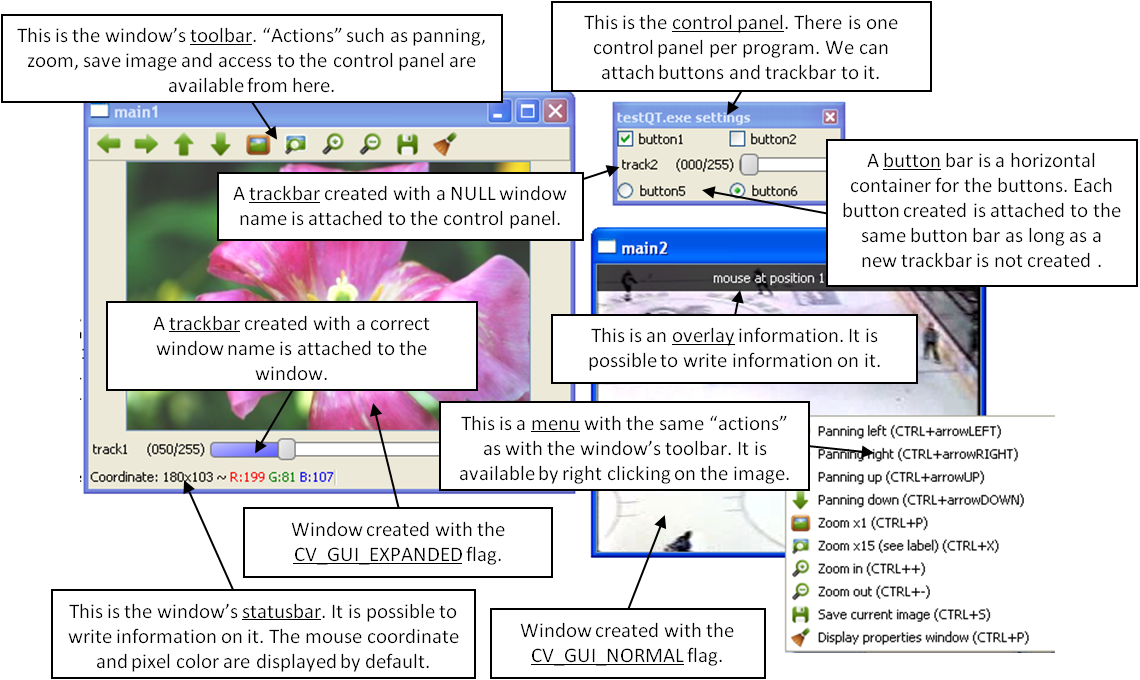
\includegraphics[width=1.1\textwidth]{pics/Qt_GUI.png}

This figure explains the new functionalities implemented with Qt GUI. As we can see, the new GUI provides a statusbar, a toolbar, and a control panel. The control panel can have trackbars and buttonbars attached to it.
\begin{itemize}
    \item  To attach a trackbar, the window\_name parameter must be NULL.
    \item  To attach a buttonbar, a button must be created. 
If the last bar attached to the control panel is a buttonbar, the new button is added on the right of the last button. 
If the last bar attached to the control panel is a trackbar, or the control panel is empty, a new buttonbar is created. Then a new button is attached to it.
\end{itemize}

The following code is an example used to generate the figure.
\begin{lstlisting}
int main(int argc, char *argv[])
    int value = 50;
    int value2 = 0;

    cvNamedWindow("main1",CV_WINDOW_NORMAL);
    cvNamedWindow("main2",CV_WINDOW_AUTOSIZE | CV_GUI_NORMAL);

    cvCreateTrackbar( "track1", "main1", &value, 255,  NULL);//OK tested
    char* nameb1 = "button1";
    char* nameb2 = "button2";
    cvCreateButton(nameb1,callbackButton,nameb1,CV_CHECKBOX,1);
	
    cvCreateButton(nameb2,callbackButton,nameb2,CV_CHECKBOX,0);
    cvCreateTrackbar( "track2", NULL, &value2, 255, NULL);
    cvCreateButton("button5",callbackButton1,NULL,CV_RADIOBOX,0);
    cvCreateButton("button6",callbackButton2,NULL,CV_RADIOBOX,1);

    cvSetMouseCallback( "main2",on_mouse,NULL );

    IplImage* img1 = cvLoadImage("files/flower.jpg");
    IplImage* img2 = cvCreateImage(cvGetSize(img1),8,3);
    CvCapture* video = cvCaptureFromFile("files/hockey.avi");
    IplImage* img3 = cvCreateImage(cvGetSize(cvQueryFrame(video)),8,3);

    while(cvWaitKey(33) != 27)
    {
        cvAddS(img1,cvScalarAll(value),img2);
        cvAddS(cvQueryFrame(video),cvScalarAll(value2),img3);
        cvShowImage("main1",img2);
        cvShowImage("main2",img3);
    }

    cvDestroyAllWindows();
    cvReleaseImage(&img1);
    cvReleaseImage(&img2);
    cvReleaseImage(&img3);
    cvReleaseCapture(&video);
    return 0;
}
\end{lstlisting}

\ifC
%CVAPI(void) cvSetWindowProperty(const char* name, int prop_id, double prop_value);
\cvCPyFunc{SetWindowProperty}
Change the parameters of the window dynamically.

\cvdefC{void  cvSetWindowProperty(const char* name, int prop\_id, double prop\_value);}

\begin{description}
\cvarg{name}{Name of the window.}
\cvarg{prop\_id}{Window's property to edit. The operation flags:
\begin{description}
\cvarg{CV\_WND\_PROP\_FULLSCREEN}{Change if the window is fullscreen (\texttt{CV\_WINDOW\_NORMAL} or \texttt{CV\_WINDOW\_FULLSCREEN}).}
\cvarg{CV\_WND\_PROP\_AUTOSIZE}{Change if the user can resize the window (texttt{CV\_WINDOW\_NORMAL} or  \texttt{CV\_WINDOW\_AUTOSIZE}).}
\cvarg{CV\_WND\_PROP\_ASPECTRATIO}{Change if the image's aspect ratio is preserved  (texttt{CV\_WINDOW\_FREERATIO} or \texttt{CV\_WINDOW\_KEEPRATIO}).}
\end{description}}
\cvarg{prop\_value}{New value of the Window's property. The operation flags:
\begin{description}
\cvarg{CV\_WINDOW\_NORMAL}{Change the window in normal size, or allows the user to resize the window.}
\cvarg{CV\_WINDOW\_AUTOSIZE}{The user cannot resize the window, the size is constrainted by the image displayed.}
\cvarg{CV\_WINDOW\_FULLSCREEN}{Change the window to fullscreen.}
\cvarg{CV\_WINDOW\_FREERATIO}{The image expends as much as it can (no ratio constraint)}
\cvarg{CV\_WINDOW\_KEEPRATIO}{The ration image is respected.}
\end{description}}
\end{description}

The function \texttt{ cvSetWindowProperty} allows to change the window's properties.



%CVAPI(double) cvGetWindowProperty(const char* name, int prop_id);
\cvCPyFunc{GetWindowProperty}
Get the parameters of the window.

\cvdefC{void  cvGetWindowProperty(const char* name, int prop\_id);}

\begin{description}
\cvarg{name}{Name of the window.}
\cvarg{prop\_id}{Window's property to retrive. The operation flags:
\begin{description}
\cvarg{CV\_WND\_PROP\_FULLSCREEN}{Change if the window is fullscreen (\texttt{CV\_WINDOW\_NORMAL} or \texttt{CV\_WINDOW\_FULLSCREEN}).}
\cvarg{CV\_WND\_PROP\_AUTOSIZE}{Change if the user can resize the window (texttt{CV\_WINDOW\_NORMAL} or  \texttt{CV\_WINDOW\_AUTOSIZE}).}
\cvarg{CV\_WND\_PROP\_ASPECTRATIO}{Change if the image's aspect ratio is preserved  (texttt{CV\_WINDOW\_FREERATIO} or \texttt{CV\_WINDOW\_KEEPRATIO}).}
\end{description}}
\end{description}
See \cross{SetWindowProperty} to know the meaning of the returned values.

The function \texttt{ cvGetWindowProperty} return window's properties.


\cvCPyFunc{FontQt}
Create the font to be used to draw text on an image (with \cross{addText}).

\cvdefC{CvFont cvFontQt(const char* nameFont, int pointSize  = -1, CvScalar color = cvScalarAll(0), int weight = CV\_FONT\_NORMAL,  int style = CV\_STYLE\_NORMAL, int spacing = 0);}

\begin{description}
\cvarg{nameFont}{Name of the font. The name should match the name of a system font (such as ``Times''). If the font is not found, a default one will be used.}
\cvarg{pointSize}{Size of the font. If not specified, equal zero or negative, the point size of the font is set to a system-dependent default value. Generally, this is 12 points.}
\cvarg{color}{Color of the font in BGRA --  A = 255 is fully transparent. Use the macro CV\_RGB for simplicity.}
\cvarg{weight}{The operation flags:
\begin{description}
\cvarg{CV\_FONT\_LIGHT}{Weight of 25}
\cvarg{CV\_FONT\_NORMAL}{Weight of 50}
\cvarg{CV\_FONT\_DEMIBOLD}{Weight of 63}
\cvarg{CV\_FONT\_BOLD}{Weight of 75}
\cvarg{CV\_FONT\_BLACK}{Weight of 87}
You can also specify a positive integer for more control.
\end{description}}
\cvarg{style}{The operation flags:
\begin{description}
\cvarg{CV\_STYLE\_NORMAL}{Font is normal}
\cvarg{CV\_STYLE\_ITALIC}{Font is in italic}
\cvarg{CV\_STYLE\_OBLIQUE}{Font is oblique}
\end{description}}
\cvarg{spacing}{Spacing between characters. Can be negative or positive}
\end{description}

The function \texttt{cvFontQt} creates a CvFont object to be used with \cross{addText}. This CvFont is not compatible with cvPutText. 

A basic usage of this function is:
\begin{lstlisting}
CvFont font = cvFontQt(''Times'');
cvAddText( img1, ``Hello World !'', cvPoint(50,50), font);
\end{lstlisting}


\cvCPyFunc{AddText}
Create the font to be used to draw text on an image 
\cvdefC{void cvAddText(const CvArr* img, const char* text, CvPoint location, CvFont *font);}

\begin{description}
\cvarg{img}{Image where the text should be drawn}
\cvarg{text}{Text to write on the image}
\cvarg{location}{Point(x,y) where the text should start on the image}
\cvarg{font}{Font to use to draw the text}
\end{description}

The function \texttt{cvAddText} draw \emph{text} on the image \emph{img} using a specific font \emph{font} (see example \cross{FontQt})


%CVAPI(void) cvDisplayOverlay(const char* name, const char* text, int delay);
\cvCPyFunc{DisplayOverlay}
Display text on the window's image as an overlay for delay milliseconds. This is not editing the image's data. The text is display on the top of the image.
\cvdefC{void cvDisplayOverlay(const char* name, const char* text, int delay);}

\begin{description}
\cvarg{name}{Name of the window}
\cvarg{text}{Overlay text to write on the window's image}
\cvarg{delay}{Delay to display the overlay text. If this function is called before the previous overlay text time out, the timer is restarted and the text updated. . If this value is zero, the text never disapers.}
\end{description}

The function \texttt{cvDisplayOverlay} aims at displaying useful information/tips on the window for a certain amount of time \emph{delay}. This information is display on the top of the window.


%CVAPI(void) cvDisplayStatusBar(const char* name, const char* text, int delayms);
\cvCPyFunc{DisplayStatusBar}
Display text on the window's statusbar as for delay milliseconds.
\cvdefC{void cvDisplayStatusBar(const char* name, const char* text, int delayms);}

\begin{description}
\cvarg{name}{Name of the window}
\cvarg{text}{Text to write on the window's statusbar}
\cvarg{delay}{Delay to display the text. If this function is called before the previous text time out, the timer is restarted and the text updated. If this value is zero, the text never disapers.}
\end{description}

The function \texttt{cvDisplayOverlay} aims at displaying useful information/tips on the window for a certain amount of time \emph{delay}. This information is displayed on the window's statubar (the window must be created with \texttt{CV\_GUI\_EXPANDED} flags).



%CVAPI(void) cvCreateOpenGLCallback( const char* window_name, CvOpenGLCallback callbackOpenGL, void* userdata CV_DEFAULT(NULL), double angle CV_DEFAULT(-1), double zmin CV_DEFAULT(-1), double zmax CV_DEFAULT(-1));
\cvCPyFunc{CreateOpenGLCallback}
Create a callback function called to draw OpenGL on top the the image display by \emph{window\_name}.
\cvdefC{void cvCreateOpenGLCallback( const char* window\_name, CvOpenGLCallback callbackOpenGL, void* userdata CV\_DEFAULT(NULL), double angle CV\_DEFAULT(-1), double zmin CV\_DEFAULT(-1), double zmax CV\_DEFAULT(-1);}

\begin{description}
\cvarg{window\_name}{Name of the window}
\cvarg{callbackOpenGL}{
Pointer to the function to be called every frame.
This function should be prototyped as \texttt{void Foo(*void);}.}
\cvarg{userdata}{pointer passed to the callback function. \emph{(Optional)}}
\cvarg{angle}{Specifies the field of view angle, in degrees, in the y direction.. \emph{(Optional - Default 45 degree)}}
\cvarg{zmin}{Specifies the distance from the viewer to the near clipping plane (always positive). \emph{(Optional - Default 0.01)}}
\cvarg{zmax}{Specifies the distance from the viewer to the far clipping plane (always positive). \emph{(Optional - Default 1000)}}    									
\end{description}

The function \texttt{cvCreateOpenGLCallback} can be used to draw 3D data on the window.  An example of callback could be:
\begin{lstlisting}
void on_opengl(void* param)
{
    //draw scene here
    glLoadIdentity();

    glTranslated(0.0, 0.0, -1.0);

    glRotatef( 55, 1, 0, 0 );
    glRotatef( 45, 0, 1, 0 );
    glRotatef( 0, 0, 0, 1 );

    static const int coords[6][4][3] = {
        { { +1, -1, -1 }, { -1, -1, -1 }, { -1, +1, -1 }, { +1, +1, -1 } },
        { { +1, +1, -1 }, { -1, +1, -1 }, { -1, +1, +1 }, { +1, +1, +1 } },
        { { +1, -1, +1 }, { +1, -1, -1 }, { +1, +1, -1 }, { +1, +1, +1 } },
        { { -1, -1, -1 }, { -1, -1, +1 }, { -1, +1, +1 }, { -1, +1, -1 } },
        { { +1, -1, +1 }, { -1, -1, +1 }, { -1, -1, -1 }, { +1, -1, -1 } },
        { { -1, -1, +1 }, { +1, -1, +1 }, { +1, +1, +1 }, { -1, +1, +1 } }
    };

    for (int i = 0; i < 6; ++i) {
                glColor3ub( i*20, 100+i*10, i*42 );
                glBegin(GL_QUADS);
                for (int j = 0; j < 4; ++j) {
                        glVertex3d(0.2 * coords[i][j][0], 0.2 * coords[i][j][1], 0.2 * coords[i][j][2]);
                }
                glEnd();
    }
}
\end{lstlisting}

\begin{lstlisting}
CV_EXTERN_C_FUNCPTR( *CvOpenGLCallback)(void* userdata));
\end{lstlisting}


%CVAPI(void) cvSaveWindowParameters(const char* name);
\cvCPyFunc{SaveWindowParameters}
Save parameters of the window \emph{window\_name}.
\cvdefC{void cvSaveWindowParameters(const char* name);}

\begin{description}
\cvarg{name}{Name of the window}							
\end{description}

The function \texttt{cvSaveWindowParameters} saves size, location, flags,  trackbars' value, zoom and panning location of the window \emph{window\_name}


%CVAPI(void) cvLoadWindowParameters(const char* name);
\cvCPyFunc{LoadWindowParameters}
Load parameters of the window \emph{window\_name}.
\cvdefC{void cvLoadWindowParameters(const char* name);}

\begin{description}
\cvarg{name}{Name of the window}							
\end{description}

The function \texttt{cvLoadWindowParameters} load size, location, flags,  trackbars' value, zoom and panning location of the window \emph{window\_name}


%CVAPI(int) cvCreateButton( const char* button_name CV_DEFAULT(NULL),CvButtonCallback on_change CV_DEFAULT(NULL), void* userdata CV_DEFAULT(NULL) , int button_type CV_DEFAULT(CV_PUSH_BUTTON), int initial_button_state CV_DEFAULT(0));
\cvCPyFunc{CreateButton}
Create a callback function called to draw OpenGL on top the the image display by \emph{window\_name}.
\cvdefC{cvCreateButton( const char* button\_name CV\_DEFAULT(NULL),CvButtonCallback on\_change CV\_DEFAULT(NULL), void* userdata CV\_DEFAULT(NULL) , int button\_type CV\_DEFAULT(CV\_PUSH\_BUTTON), int initial\_button\_state CV\_DEFAULT(0);}

\begin{description}
\cvarg{ button\_name}{Name of the button  \emph{( if NULL, the name will be "button <number of boutton>")}}
\cvarg{on\_change}{
Pointer to the function to be called every time the button changed its state.
This function should be prototyped as \texttt{void Foo(int state,*void);}. \emph{state} is the current state of the button. It could be -1 for a push button, 0 or 1 for a check/radio box button.}
\cvarg{userdata}{pointer passed to the callback function. \emph{(Optional)}}
\end{description}

The \texttt{button\_type} parameter can be :  \emph{(Optional -- Will be a push button by default.)
\begin{description}
\cvarg{CV\_PUSH\_BUTTON}{The button will be a push button.}
\cvarg{CV\_CHECKBOX}{The button will be a checkbox button.}
\cvarg{CV\_RADIOBOX}{The button will be a radiobox button. The radiobox on the same buttonbar (same line) are exclusive; one on can be select at the time.}
\end{description}}	
\begin{description}
\cvarg{initial\_button\_state}{Default state of the button. Use for checkbox and radiobox, its value could be 0 or 1. \emph{(Optional)}}							
\end{description}

The function \texttt{cvCreateButton} attach button to the control panel. Each button is added to a buttonbar on the right of the last button.
A new buttonbar is create if nothing was attached to the control panel before, or if the last element attached to the control panel was a trackbar.

Here are various example of \texttt{cvCreateButton}  function call:
\begin{lstlisting}
cvCreateButton(NULL,callbackButton);//create a push button "button 0", that will call callbackButton. 
cvCreateButton("button2",callbackButton,NULL,CV\_CHECKBOX,0);
cvCreateButton("button3",callbackButton,&value);
cvCreateButton("button5",callbackButton1,NULL,CV\_RADIOBOX);
cvCreateButton("button6",callbackButton2,NULL,CV\_PUSH\_BUTTON,1);
\end{lstlisting}

\begin{lstlisting}
CV_EXTERN_C_FUNCPTR( *CvButtonCallback)(int state, void* userdata));
\end{lstlisting}

\fi





\ifCpp


%CVAPI(void) cvSetWindowProperty(const char* name, int prop_id, double prop_value);
\cvCppFunc{setWindowProperty}
Change the parameters of the window dynamically.

\cvdefCpp{void  setWindowProperty(const string\& name, int prop\_id, double prop\_value);}

\begin{description}
\cvarg{name}{Name of the window.}
\cvarg{prop\_id}{Window's property to edit. The operation flags:
\begin{description}
\cvarg{CV\_WND\_PROP\_FULLSCREEN}{Change if the window is fullscreen (\texttt{CV\_WINDOW\_NORMAL} or \texttt{CV\_WINDOW\_FULLSCREEN}).}
\cvarg{CV\_WND\_PROP\_AUTOSIZE}{Change if the user can resize the window (texttt{CV\_WINDOW\_NORMAL} or  \texttt{CV\_WINDOW\_AUTOSIZE}).}
\cvarg{CV\_WND\_PROP\_ASPECTRATIO}{Change if the image's aspect ratio is preserved  (texttt{CV\_WINDOW\_FREERATIO} or \texttt{CV\_WINDOW\_KEEPRATIO}).}
\end{description}}
\cvarg{prop\_value}{New value of the Window's property. The operation flags:
\begin{description}
\cvarg{CV\_WINDOW\_NORMAL}{Change the window in normal size, or allows the user to resize the window.}
\cvarg{CV\_WINDOW\_AUTOSIZE}{The user cannot resize the window, the size is constrainted by the image displayed.}
\cvarg{CV\_WINDOW\_FULLSCREEN}{Change the window to fullscreen.}
\cvarg{CV\_WINDOW\_FREERATIO}{The image expends as much as it can (no ratio constraint)}
\cvarg{CV\_WINDOW\_KEEPRATIO}{The ration image is respected.}
\end{description}}
\end{description}

The function \texttt{ setWindowProperty} allows to change the window's properties.



%CVAPI(double) cvGetWindowProperty(const char* name, int prop_id);
\cvCppFunc{getWindowProperty}
Get the parameters of the window.

\cvdefCpp{void  getWindowProperty(const char* name, int prop\_id);}

\begin{description}
\cvarg{name}{Name of the window.}
\cvarg{prop\_id}{Window's property to retrive. The operation flags:
\begin{description}
\cvarg{CV\_WND\_PROP\_FULLSCREEN}{Change if the window is fullscreen (\texttt{CV\_WINDOW\_NORMAL} or \texttt{CV\_WINDOW\_FULLSCREEN}).}
\cvarg{CV\_WND\_PROP\_AUTOSIZE}{Change if the user can resize the window (texttt{CV\_WINDOW\_NORMAL} or  \texttt{CV\_WINDOW\_AUTOSIZE}).}
\cvarg{CV\_WND\_PROP\_ASPECTRATIO}{Change if the image's aspect ratio is preserved  (texttt{CV\_WINDOW\_FREERATIO} or \texttt{CV\_WINDOW\_KEEPRATIO}).}
\end{description}}
\end{description}
See \cross{setWindowProperty} to know the meaning of the returned values.

The function \texttt{ getWindowProperty} return window's properties.


\cvCppFunc{fontQt}
Create the font to be used to draw text on an image.

\cvdefCpp{CvFont fontQt(const string\& nameFont, int pointSize  = -1, Scalar color = Scalar::all(0), int weight = CV\_FONT\_NORMAL,  int style = CV\_STYLE\_NORMAL, int spacing = 0);}

\begin{description}
\cvarg{nameFont}{Name of the font. The name should match the name of a system font (such as ``Times''). If the font is not found, a default one will be used.}
\cvarg{pointSize}{Size of the font. If not specified, equal zero or negative, the point size of the font is set to a system-dependent default value. Generally, this is 12 points.}
\cvarg{color}{Color of the font in BGRA --  A = 255 is fully transparent. Use the macro CV\_RGB for simplicity.}
\cvarg{weight}{The operation flags:
\begin{description}
\cvarg{CV\_FONT\_LIGHT}{Weight of 25}
\cvarg{CV\_FONT\_NORMAL}{Weight of 50}
\cvarg{CV\_FONT\_DEMIBOLD}{Weight of 63}
\cvarg{CV\_FONT\_BOLD}{Weight of 75}
\cvarg{CV\_FONT\_BLACK}{Weight of 87}
You can also specify a positive integer for more control.
\end{description}}
\cvarg{style}{The operation flags:
\begin{description}
\cvarg{CV\_STYLE\_NORMAL}{Font is normal}
\cvarg{CV\_STYLE\_ITALIC}{Font is in italic}
\cvarg{CV\_STYLE\_OBLIQUE}{Font is oblique}
\end{description}}
\cvarg{spacing}{Spacing between characters. Can be negative or positive}
\end{description}

The function \texttt{fontQt} creates a CvFont object. This CvFont is not compatible with putText. 

A basic usage of this function is:
\begin{lstlisting}
CvFont font = fontQt(''Times'');
addText( img1, ``Hello World !'', Point(50,50), font);
\end{lstlisting}

\cvCppFunc{addText}
Create the font to be used to draw text on an image 
\cvdefCpp{void addText(const Mat\& img, const string\& text, Point location, CvFont *font);}

\begin{description}
\cvarg{img}{Image where the text should be drawn}
\cvarg{text}{Text to write on the image}
\cvarg{location}{Point(x,y) where the text should start on the image}
\cvarg{font}{Font to use to draw the text}
\end{description}

The function \texttt{addText} draw \emph{text} on the image \emph{img} using a specific font \emph{font} (see example \cross{fontQt})


%CVAPI(void) cvDisplayOverlay(const char* name, const char* text, int delay);
\cvCppFunc{displayOverlay}
Display text on the window's image as an overlay for delay milliseconds. This is not editing the image's data. The text is display on the top of the image.
\cvdefCpp{void displayOverlay(const string\& name, const string\& text, int delay);}

\begin{description}
\cvarg{name}{Name of the window}
\cvarg{text}{Overlay text to write on the window's image}
\cvarg{delay}{Delay to display the overlay text. If this function is called before the previous overlay text time out, the timer is restarted and the text updated. . If this value is zero, the text never disapers.}
\end{description}

The function \texttt{displayOverlay} aims at displaying useful information/tips on the window for a certain amount of time \emph{delay}. This information is display on the top of the window.


%CVAPI(void) cvDisplayStatusBar(const char* name, const char* text, int delayms);
\cvCppFunc{displayStatusBar}
Display text on the window's statusbar as for delay milliseconds.
\cvdefCpp{void displayStatusBar(const string\& name, const string\& text, int delayms);}

\begin{description}
\cvarg{name}{Name of the window}
\cvarg{text}{Text to write on the window's statusbar}
\cvarg{delay}{Delay to display the text. If this function is called before the previous text time out, the timer is restarted and the text updated. If this value is zero, the text never disapers.}
\end{description}

The function \texttt{displayOverlay} aims at displaying useful information/tips on the window for a certain amount of time \emph{delay}. This information is displayed on the window's statubar (the window must be created with \texttt{CV\_GUI\_EXPANDED} flags).



%CVAPI(void) cvCreateOpenGLCallback( const char* window_name, CvOpenGLCallback callbackOpenGL, void* userdata CV_DEFAULT(NULL), double angle CV_DEFAULT(-1), double zmin CV_DEFAULT(-1), double zmax CV_DEFAULT(-1));
\cvCppFunc{createOpenGLCallback}
Create a callback function called to draw OpenGL on top the the image display by \emph{window\_name}.
\cvdefCpp{void createOpenGLCallback( const string\& window\_name, OpenGLCallback callbackOpenGL, void* userdata CV\_DEFAULT(NULL), double angle CV\_DEFAULT(-1), double zmin CV\_DEFAULT(-1), double zmax CV\_DEFAULT(-1);}

\begin{description}
\cvarg{window\_name}{Name of the window}
\cvarg{callbackOpenGL}{
Pointer to the function to be called every frame.
This function should be prototyped as \texttt{void Foo(*void);}.}
\cvarg{userdata}{pointer passed to the callback function. \emph{(Optional)}}
\cvarg{angle}{Specifies the field of view angle, in degrees, in the y direction.. \emph{(Optional - Default 45 degree)}}
\cvarg{zmin}{Specifies the distance from the viewer to the near clipping plane (always positive). \emph{(Optional - Default 0.01)}}
\cvarg{zmax}{Specifies the distance from the viewer to the far clipping plane (always positive). \emph{(Optional - Default 1000)}}    									
\end{description}

The function \texttt{createOpenGLCallback} can be used to draw 3D data on the window.  An example of callback could be:
\begin{lstlisting}
void on_opengl(void* param)
{
    glLoadIdentity();

    glTranslated(0.0, 0.0, -1.0);

    glRotatef( 55, 1, 0, 0 );
    glRotatef( 45, 0, 1, 0 );
    glRotatef( 0, 0, 0, 1 );

    static const int coords[6][4][3] = {
        { { +1, -1, -1 }, { -1, -1, -1 }, { -1, +1, -1 }, { +1, +1, -1 } },
        { { +1, +1, -1 }, { -1, +1, -1 }, { -1, +1, +1 }, { +1, +1, +1 } },
        { { +1, -1, +1 }, { +1, -1, -1 }, { +1, +1, -1 }, { +1, +1, +1 } },
        { { -1, -1, -1 }, { -1, -1, +1 }, { -1, +1, +1 }, { -1, +1, -1 } },
        { { +1, -1, +1 }, { -1, -1, +1 }, { -1, -1, -1 }, { +1, -1, -1 } },
        { { -1, -1, +1 }, { +1, -1, +1 }, { +1, +1, +1 }, { -1, +1, +1 } }
    };

    for (int i = 0; i < 6; ++i) {
                glColor3ub( i*20, 100+i*10, i*42 );
                glBegin(GL_QUADS);
                for (int j = 0; j < 4; ++j) {
                        glVertex3d(0.2 * coords[i][j][0], 0.2 * coords[i][j][1], 0.2 * coords[i][j][2]);
                }
                glEnd();
    }
}
\end{lstlisting}


%CVAPI(void) cvSaveWindowParameters(const char* name);
\cvCppFunc{saveWindowParameters}
Save parameters of the window \emph{window\_name}.
\cvdefCpp{void saveWindowParameters(const string\& name);}

\begin{description}
\cvarg{name}{Name of the window}							
\end{description}

The function \texttt{saveWindowParameters} saves size, location, flags,  trackbars' value, zoom and panning location of the window \emph{window\_name}


%CVAPI(void) cvLoadWindowParameters(const char* name);
\cvCppFunc{loadWindowParameters}
Load parameters of the window \emph{window\_name}.
\cvdefCpp{void loadWindowParameters(const string\& name);}

\begin{description}
\cvarg{name}{Name of the window}							
\end{description}

The function \texttt{loadWindowParameters} load size, location, flags,  trackbars' value, zoom and panning location of the window \emph{window\_name}


%CVAPI(int) cvCreateButton( const char* button_name CV_DEFAULT(NULL),CvButtonCallback on_change CV_DEFAULT(NULL), void* userdata CV_DEFAULT(NULL) , int button_type CV_DEFAULT(CV_PUSH_BUTTON), int initial_button_state CV_DEFAULT(0));
\cvCppFunc{createButton}
Create a callback function called to draw OpenGL on top the the image display by \emph{window\_name}.
\cvdefCpp{createButton( const string\& button\_name CV\_DEFAULT(NULL),ButtonCallback on\_change CV\_DEFAULT(NULL), void* userdata CV\_DEFAULT(NULL) , int button\_type CV\_DEFAULT(CV\_PUSH\_BUTTON), int initial\_button\_state CV\_DEFAULT(0);}

\begin{description}
\cvarg{ button\_name}{Name of the button  \emph{( if NULL, the name will be "button <number of boutton>")}}
\cvarg{on\_change}{
Pointer to the function to be called every time the button changed its state.
This function should be prototyped as \texttt{void Foo(int state,*void);}. \emph{state} is the current state of the button. It could be -1 for a push button, 0 or 1 for a check/radio box button.}
\cvarg{userdata}{pointer passed to the callback function. \emph{(Optional)}}
\end{description}

The \texttt{button\_type} parameter can be :  \emph{(Optional -- Will be a push button by default.)
\begin{description}
\cvarg{CV\_PUSH\_BUTTON}{The button will be a push button.}
\cvarg{CV\_CHECKBOX}{The button will be a checkbox button.}
\cvarg{CV\_RADIOBOX}{The button will be a radiobox button. The radiobox on the same buttonbar (same line) are exclusive; one on can be select at the time.}
\end{description}}	
\begin{description}
\cvarg{initial\_button\_state}{Default state of the button. Use for checkbox and radiobox, its value could be 0 or 1. \emph{(Optional)}}							
\end{description}

The function \texttt{createButton} attach a button to the control panel. Each button is added to a buttonbar on the right of the last button.
A new buttonbar is create if nothing was attached to the control panel before, or if the last element attached to the control panel was a trackbar.

Here are various example of \texttt{createButton}  function call:
\begin{lstlisting}
createButton(NULL,callbackButton);//create a push button "button 0", that will call callbackButton. 
createButton("button2",callbackButton,NULL,CV\_CHECKBOX,0);
createButton("button3",callbackButton,&value);
createButton("button5",callbackButton1,NULL,CV\_RADIOBOX);
createButton("button6",callbackButton2,NULL,CV\_PUSH\_BUTTON,1);
\end{lstlisting}

\fi